\documentclass[a4]{beamer}
\usepackage{amssymb}
\usepackage{graphicx}
\usepackage{subfigure}
\usepackage{newlfont}
\usepackage{amsmath,amsthm,amsfonts}
%\usepackage{beamerthemesplit}
\usepackage{pgf,pgfarrows,pgfnodes,pgfautomata,pgfheaps,pgfshade}
\usepackage{mathptmx} % Font Family
\usepackage{helvet} % Font Family
\usepackage{color}
\mode<presentation> {
	\usetheme{Default} % was Frankfurt
	\useinnertheme{rounded}
	\useoutertheme{infolines}
	\usefonttheme{serif}
	%\usecolortheme{wolverine}
	% \usecolortheme{rose}
	\usefonttheme{structurebold}
}
\setbeamercovered{dynamic}
\title[MA4413]{Statistics for Computing \\ {\normalsize MA4413 Lecture 11A}}
\author[Kevin O'Brien]{Kevin O'Brien \\ {\scriptsize kevin.obrien@ul.ie}}
\date{Autumn 2012}
\institute[Maths \& Stats]{Dept. of Mathematics \& Statistics, \\ University \textit{of} Limerick}
\renewcommand{\arraystretch}{1.5}
%------------------------------------------------------------------------%
\begin{document}
\begin{frame}
\frametitle{Mutual Information}
Mutual information is one of many quantities that measures how much one random variables gives about another. It is a dimensionless quantity. Mutual Informaiton can be thought of as the reduction in uncertainty about one random variable given knowledge of another. 
\begin{itemize}\item High mutual information indicates a large reduction in uncertainty, \item low mutual information indicates a small reduction, \item  zero mutual information between two random variables means the variables are independent.
\end{itemize}
Efficient communication systems have high mutual information.
\end{frame}
%---------------------------------------------------------------------------------------------------------------------------------------%
\begin{frame}
\frametitle{Mutual Information}
\vspace{-1cm}
\textbf{Joint Entropies:}\\
Using the input probabilities $P(x_i)$, output probabilities $P(y_i)$, transition probabilities $P(y_i|x_i)$,
and joint probabilities $P(x_i,y_j)$, we can define the following various entropy functions for a channel
with m inputs and n outputs:

\begin{itemize}
\item $H(X) = - \sum ^{m}_{i=1} P(x_i) \mbox{log}_2 P(x_i)$%; P(x;) (10.21)
\item $H(Y) = - \sum ^{n}_{j=1} P(y_j) \mbox{log}_2 P(y_j)$
\item $H(X, Y)= - \sum ^{n}_{j=1}\sum ^{m}_{i=1} P(x_i,y_j) \mbox{log}_2 P(x_i,y_j)$
\end{itemize}
\end{frame}

%---------------------------------------------------------------------------------------------------------------------------------------%
\begin{frame}
\frametitle{Mutual Information: Joint Entropy}
\vspace{-1cm}
These entropies can be interpreted as follows:\begin{itemize}\item $ H(X)$ is the average uncertainty of the channel input,
and $H(Y)$ is the average uncertainty of the channel output.\item  The joint entropy $H(X,Y)$ is the average uncertainty of the communication channel as a
whole.\end{itemize}
\end{frame}
%---------------------------------------------------------------------------------------------------------------------------------------%
\begin{frame}
\frametitle{Mutual Information: Conditional Entropy}
\begin{itemize}
\item The conditional entropy $H(X|Y)$ is a
measure of the average uncertainty remaining about the channel input after the channel output has
been observed. \item This is sometimes called the equivocation of X with respect to Y.  \item The
conditional entropy $H(Y|X)$ is the average uncertainty of the channel output given that X was
transmitted.
\end{itemize}
\begin{itemize}
\item $H(X|Y)= - \sum ^{n}_{j=1}\sum ^{m}_{i=1} P(x_i,y_j) \mbox{log}_2 P(x_i|y_j)$
\item $H(Y|X)= - \sum ^{n}_{j=1}\sum ^{m}_{i=1} P(x_i,y_j) \mbox{log}_2 P(y_j|x_i)$
\end{itemize}
\end{frame}
%-----------------------------------------------------------------------------------------------%
\begin{frame}
\frametitle{Mutual Information : Useful Identities}
Two useful relationships among the types of entropies are
\begin{itemize}
\item $H(X,Y)=H(X|Y)+H(Y) $
\item $H(X,Y)=H(Y|X)+H(X) $
\end{itemize}
(Remark : compare to identities in probability theory)
\end{frame}
%-----------------------------------------------------------------------------------------------%
\begin{frame}
\frametitle{Mutual Information : Useful Identities}
\begin{figure}
\centering
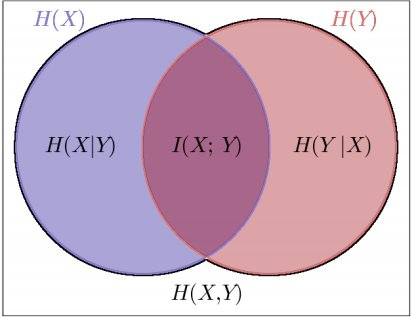
\includegraphics[width=0.7\linewidth]{images/11BMutualInfo}
\caption{}
\label{fig:11BMutualInfo}
\end{figure}


\end{frame}



\begin{frame}

\frametitle{Mutual Information}
The mutual information $I(X; Y)$ of a channel is defined by
\[ I(X; Y) = H(X) -  H(X|Y) \mbox{    (b/symbol) } \]

Alternatively we can define it as either
\[ I(X; Y) = H(Y) -  H(Y|X) \mbox{     (b/symbol) } \]
 or as
\[ I(X; Y) = H(Y)+ H(Y)  - H(X,Y) \mbox{    (b/symbol) } \]
Remark: The
mutual information is the reduction of
entropy of X when Y
is
known.
\end{frame}

%----------------------------------------------------------------------------------%
\frame{
\frametitle{Entropy: some remarks}
\begin{itemize}
\item Entropy is the uncertainty of a single random variable. \item We can define \textbf{\emph{conditional entropy }}$H(X|Y)$, which is the entropy of a random variable
conditional on the knowledge of another random variable. \item The reduction in uncertainty due to another random variable is called the \textbf{\emph{mutual information}}.
\end{itemize}
}
%----------------------------------------------------------------------------------%
\begin{frame}
\frametitle{Entropies: Example}
\begin{itemize}
\item The input source to a noisy communication channel is a random variable X over the
four symbols $\{a, b, c, d\}$. \item  The output from this channel is a random variable Y over these same
four symbols.
\end{itemize}

\end{frame}
%----------------------------------------------------------------Part 2 %
\begin{frame}
\frametitle{Entropies: Example}
The joint distribution of these two random variables is as follows:\\ \bigskip
\begin{center}
\begin{tabular}{|c|c|c|c|c|}
\hline
&x=a& x=b & x=c & x=d \\ \hline
y=b &1/8 &1/16 &1/16 &1/4 \\ \hline
y=b &1/16 & 1/8& 1/16& 0 \\ \hline
y=c & 1/32&1/32 & 1/16 & 0\\ \hline
y=d & 1/32& 1/32& 1/16 & 0\\ \hline \hline
\end{tabular}
\end{center}
\end{frame}
%----------------------------------------------------------------Part 2 %
\begin{frame}
\frametitle{Entropies: Example}
\begin{itemize}
\item Write down the marginal distribution for $X$ and compute the marginal entropy $H(X)$.
\item Write down the marginal distribution for $Y$ and compute the marginal entropy $H(Y )$.
\item (next class) What is the joint entropy $H(X, Y ) $ of the two random variables?
\item (next class) What is the conditional entropy $H(Y|X)$?
\item (next class) What is the conditional entropy $H(X|Y)$?
\item (next class) What is the mutual information $I(X;Y)$ between the two random variables?
\end{itemize}
\end{frame}
%----------------------------------------------------------------------------------%
%----------------------------------------------------------------Part 2 %
\begin{frame}
\frametitle{Entropies: Example}
The marginal distribution of these two random variables is as follows:\\ \bigskip
\begin{center}
\begin{tabular}{|c|c|c|c|c||c|}
\hline
&x=a& x=b & x=c & x=d &\alert{P(Y)}\\ \hline
y=b &1/8 &1/16 &1/16 &1/4 & \alert{0.50}\\ \hline
y=b &1/16 & 1/8& 1/16& 0 & \alert{0.25}\\ \hline
y=c & 1/32&1/32 & 1/16 & 0& \alert{0.125}\\ \hline
y=d & 1/32& 1/32& 1/16 & 0& \alert{0.125}\\ \hline \hline
\alert{P(X)} & \alert{0.25}& \alert{0.25}& \alert{0.25} & \alert{0.25}&\\ \hline
\end{tabular}
\end{center}
\end{frame}


\begin{frame}
\frametitle{Entropies: Example}
\begin{itemize}

\item H(X) , the entropy of X, is computed as\\
 \[H(X) = -\sum P(x_i) \mbox{log}_2P(x_i)\] \item $H(X) =  (-0.25 \times -2) + (-0.25 \times -2) +(-0.25 \times -2) +(-0.25 \times -2)$\item $ H(X) = 2 \mbox{b}$ \bigskip

\item H(X) , the entropy of Y, is computed as\\
 \[H(Y) = -\sum P(y_j) \mbox{log}_2P(y_j)\] \item $H(Y) =  (-0.5 \times -1) +(-0.25 \times -2)  + (-0.125 \times -3)  +(-0.125 \times -3)$\item $ H(Y) = 1.75 \mbox{b}$


\end{itemize}
\end{frame}


\end{document}
\end{document}